\section{Pressure driven flows}
\label{sec:dsmc_pressure_driven_flows}
In order to induce flow in a system, it is common to apply a pressure gradient. A constant pressure gradient means that there acts a nonzero net force on any volume element $dV$ in the system. There might be regions where the net force \textit{is} zero, but on average, the simulated substance feels a force. In continuum models, the pressure, and hence pressure gradients, is often incorporated as boundary conditions where pressure is specified at given points. In particle models like DSMC, pressure must be defined through statistical mechanics and is actually not a required property. This is fairly obvious, because the knowledge of a consept like pressure should not change the rules of physics. The universe itself does not care about whether or not we have figured out what pressure is, but it is a convenient mathematical tool for us.

\subsection{What is pressure?}
The usual definition of pressure is the one from classical mechanics; force per area
\begin{align}
	P = \frac{F}{A}.
\end{align}
In statistical mechanics, the pressure is defined in a statistical manner through the entropy
\begin{align}
	P = T\left(\dpart{S}{V}\right)_{U,N},
\end{align}
which is the mathematical way to say \textit{pressure is the thing that is equal in two systems if they can exchange volume}. 

\subsection{Acceleration-driven flow}
We will use the ideas of continuum mechanics to derive a relation between the pressure gradient $\nabla P$ and a constant force $F$ (often called gravity), where the latter will be used to induce flow in the DSMC-algorithm. We look at a volume element of size $\Delta x\Delta y\Delta z$ in a channel with a continuous fluid and a pressure gradient in the $x$-direction, see figure \ref{fig:pressure_gravity_equivalent}. The force acting on the volume element from the pressure gradient is
\begin{align}
	F_x = P_1\Delta y\Delta z - P_2\Delta y\Delta z = \Delta y\Delta z\Delta P,
\end{align}
where $\Delta P = P_1 - P_2$. We aim to find a constant force $F_x=ma_x$ being equivalent to that of the pressure difference. With an applied acceleration $g$, the force is then
\begin{align}
	F_x = mg = \rho_m \Delta V g = \Delta y\Delta z\Delta P = \Delta V \frac{\Delta P}{\Delta x},
\end{align}
which gives the relation
\begin{align}
	g = \frac{\Delta P}{\rho_m\Delta x}
\end{align}
or solved for the pressure difference
\begin{align}
	\label{eq:acceleration_to_pressure_difference}
	\Delta P = \rho_m g \Delta x.
\end{align}
This is the approach we have used to induce flow in the DSMC code, and the implementation is shown in listing \ref{lst:acceleration_driven_flow}.
\begin{lstlisting}[caption=Acceleration of particles in the DSMC code., label=lst:acceleration_driven_flow]
void System::accelerate(double acceleration, int flow_direction) {
    for(int n=0;n<num_molecules;n++) {
        v.at(3*n+flow_direction) += acceleration;
    }
}
\end{lstlisting}

\subsection{Limitations}
One problem with this approach appears if the path through a system has larger parts in the opposite direction of the pressure difference, see figure \ref{fig:gravity_problem}. If the system is driven by a real pressure difference, the net force on a volume element in the gray area would differ both in magnitude and direction.
\begin{figure}[h]
\begin{center}
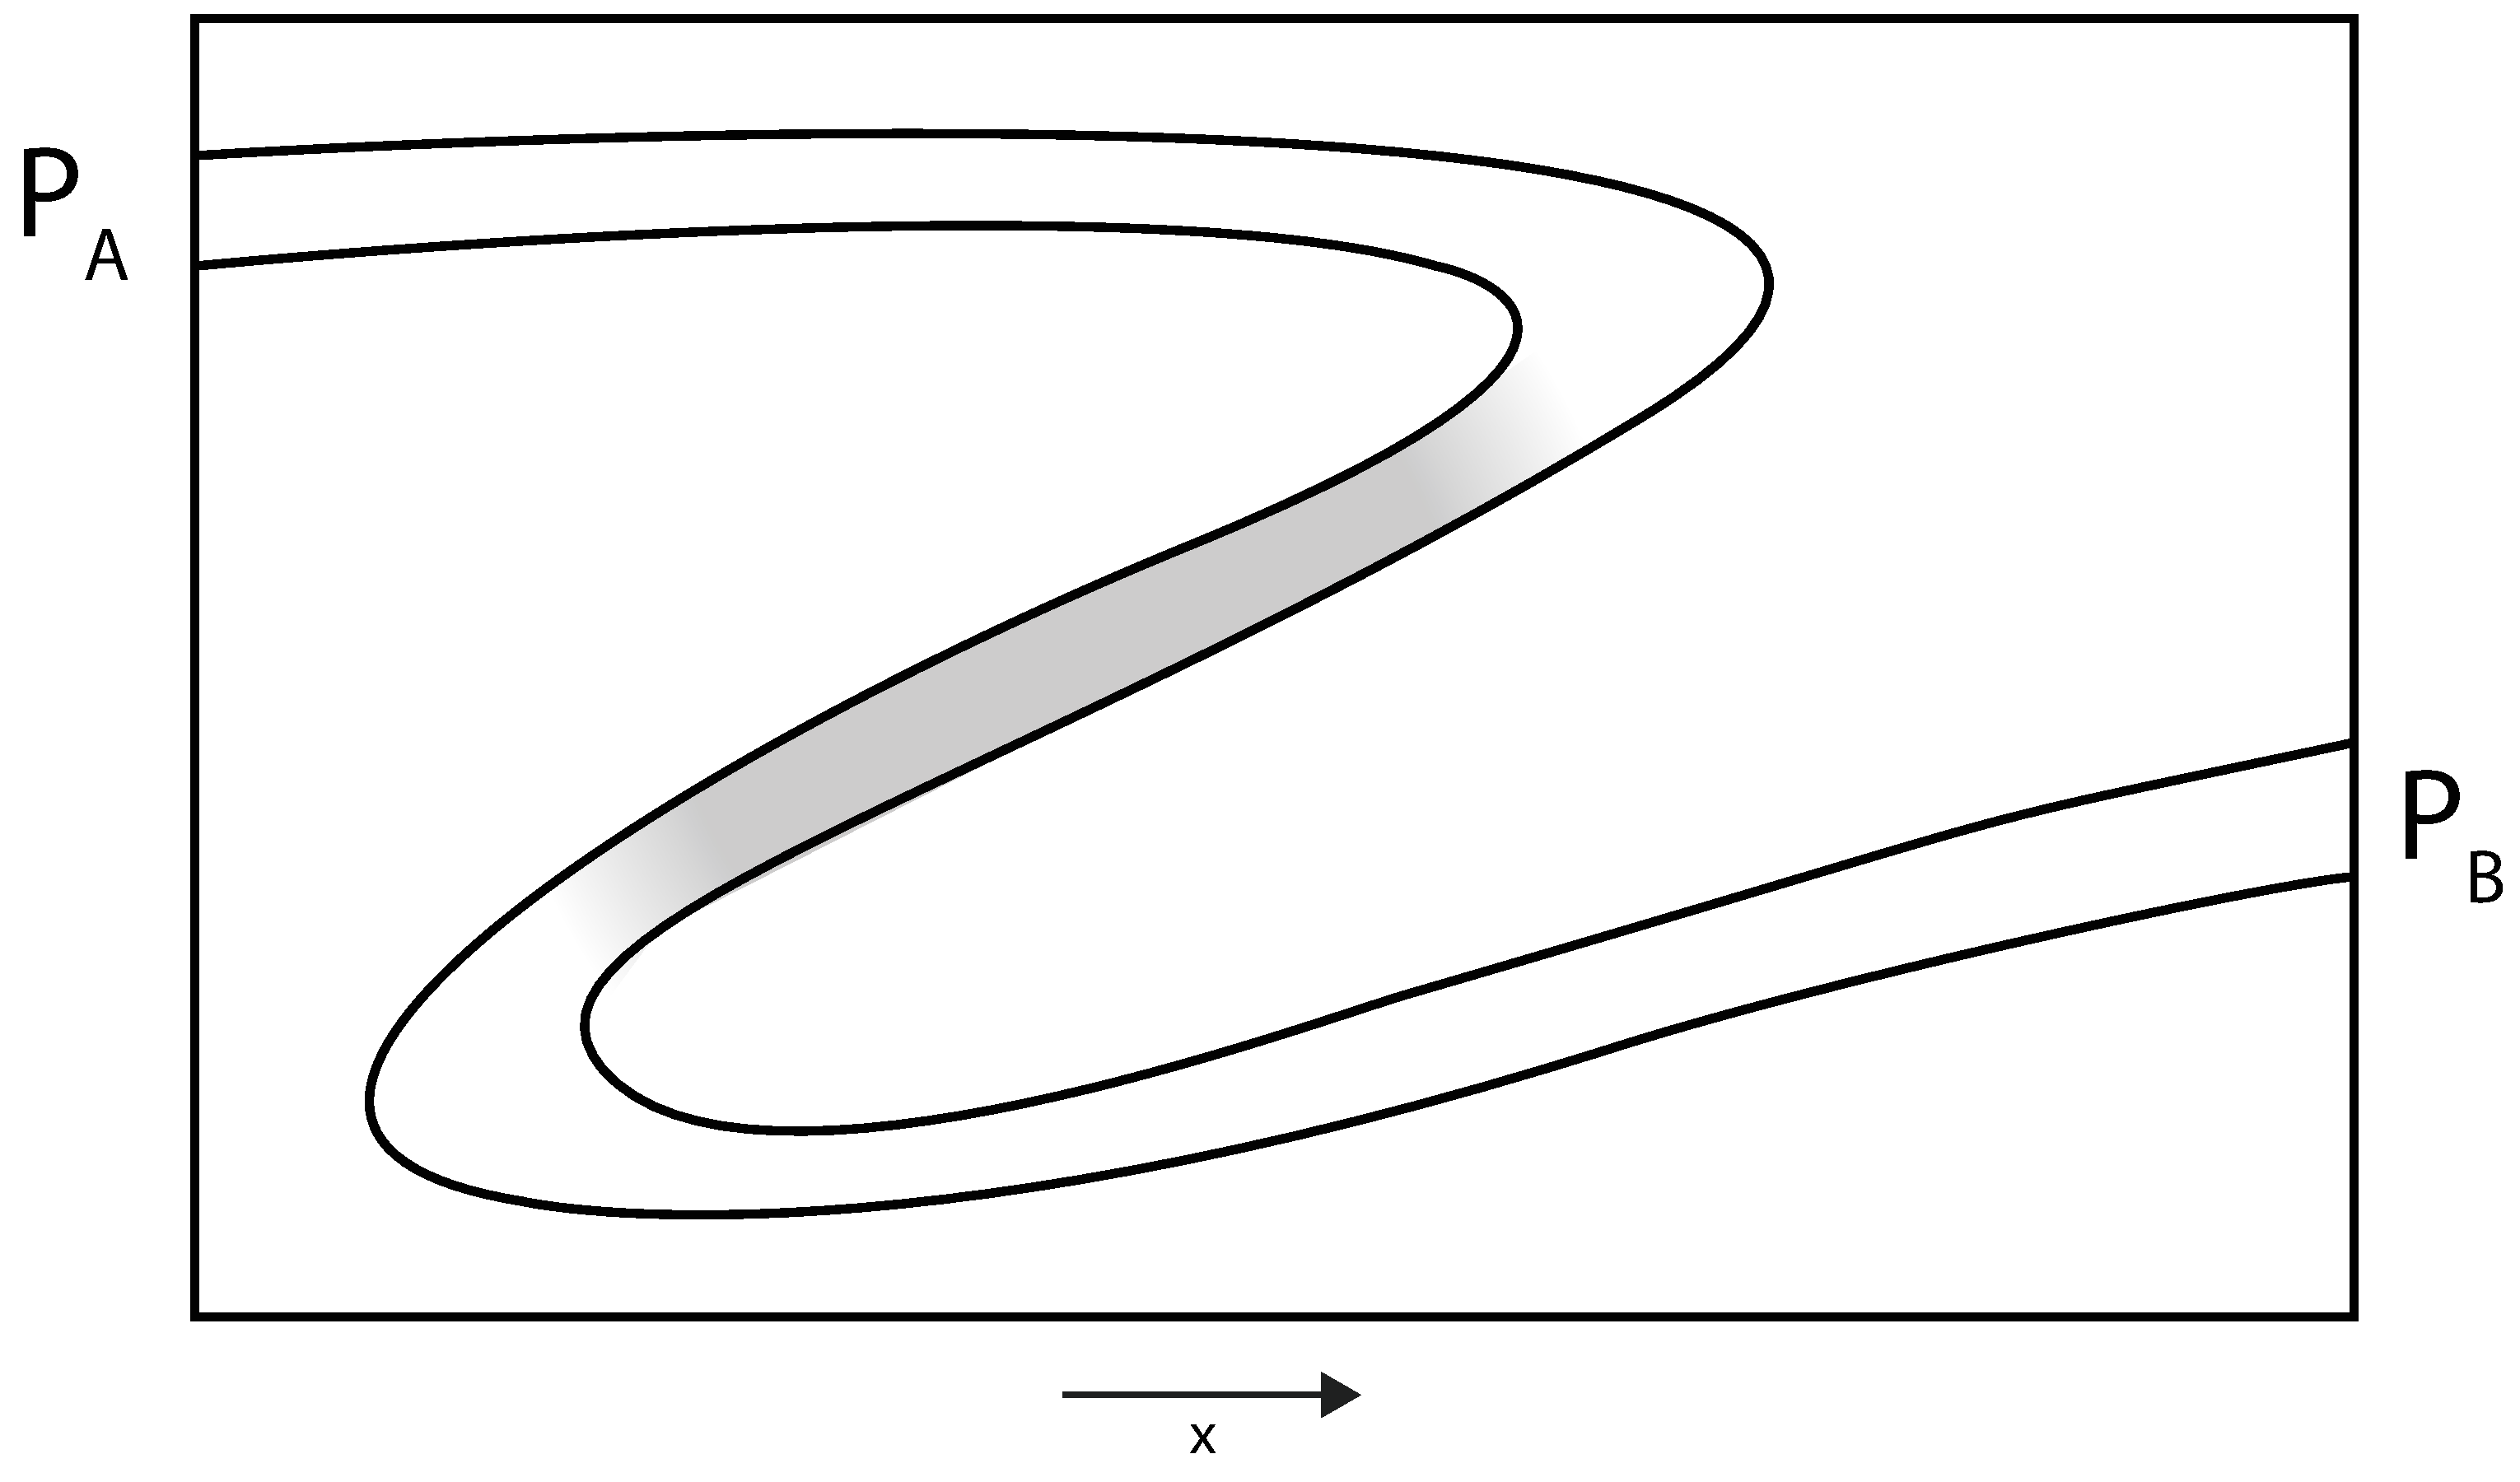
\includegraphics[width=0.7\textwidth, trim=0cm 0cm 0cm 0cm, clip]{DSMC/figures/gravity_problem.eps}
\end{center}
\caption{Acceleration-driven flows will not reproduce correct results when the gas in a large part (marked gray) of the channel will flow in the opposite direction of the pressure gradient.}
\label{fig:gravity_problem}
\end{figure}

\subsection{Measuring permeability}
\label{sec:permeability_acceleration_driven}
The permeability was defined in section \ref{sec:permeability_dsmc} through Darcy's law
\begin{align}
	k = Q{2PL\mu\over A\left(P_L^2 - P_0^2\right)},
\end{align}
but we did not know how to correctly evaluate the pressure since $x=0$ is the same point as $x=L$ in a periodic system with length $L$. We can define the pressure at $x=0$ through the ideal gas law, and due to the acceleration $g$ there is an implied pressure at $x=L$ we can find by using equation \eqref{eq:acceleration_to_pressure_difference}
\begin{align}
	P_0 &= \rho_n(x=0)kT\\
	P_L &= P_0 - \Delta P \\
	&= \rho_n(x=0)kT - \bar{\rho}_m g L,
\end{align}
where $\bar{\rho}_m$ is the average density in the system and we have used that $\Delta x=L$.\\
We still need to figure out how to measure the volumetric flow rate $Q$. The volumetric flow rate tells us how much volume that passes through a surface per time. The simplest way to measure $Q$ is to count how many particles that have passed through a surface and multiply that number with the volume per particle $\rho_n^{-1}$. Since we apply periodic boundary conditions on particles that fly out of the system, we just have to keep track of how many, this is illustrated in listing \ref{lst:dsmc_apply_periodic_boundary_conditions}.
\begin{lstlisting}[caption=Example of how to apply periodic boundary conditions and at the same time calculate number flux., label=lst:dsmc_apply_periodic_boundary_conditions]
void apply_periodic_boundary_conditions(vector<double>&position, vector<long> &count_periodic, vector<double> &system_length)
{
    if(position[0] >= system_length[0]) { 
    	position[0] -= system_length[0]; count_periodic[0]++; 
    }
    else if(position[0] < 0) { 
    	position[0] += system_length[1]; count_periodic[0]--; 
    }

    if(position[1] >= system_length[1]) { 
    	position[1] -= system_length[1]; count_periodic[1]++;
    }
    else if(position[1] < 0) {
    	position[1] += system_length[1]; count_periodic[1]--; 
    }

    if(position[2] >= system_length[2]) { 
    	position[2] -= system_length[2]; count_periodic[2]++; 
    }
    else if(position[2] < 0) {
    	position[2] += system_length[2]; count_periodic[2]--; 
    }
}
\end{lstlisting}
Now that we have the number flux, we can easily calculate the permeability as shown in listing 
\begin{lstlisting}[caption=Calculation of permeability\, assuming that flow is in the $z$-direction., label=lst:dsmc_permeability]
double calculate_permeability(double volume, long num_particles, double viscosity, vector<long> &count_periodic, vector<double> &system_length, double mass_density, double acceleration)
{	
    double volume_per_particle = volume / num_particles;

    // We assuming that the flow is in z-direction
    double volume_flow_rate = count_periodic[2]*volume_per_molecule;
    double area = system_length[0]*system_length[1];

    double pressure_0 = system->density*system->temperature;
    double pressure_L = pressure_in_reservoir_0 - mass_density*acceleration*system_length[2];
    double permeability = 2*pressure_0*volume_flow_rate*system_length[2]*viscosity / (area * (pressure_0*pressure_0 - pressure_L*pressure_L));

    return permeability;
}
\end{lstlisting}